% !TEX encoding = UTF-8
% !TEX TS-program = pdflatex
% !TEX root = ../tesi.tex

%**************************************************************
\chapter{Resoconto dello stage}
\label{cap:resoconto-stage}
%**************************************************************

%**************************************************************
\section{Pianificazione}
Prima dell'inizio del progetto di stage, insieme al mio tutor aziendale, abbiamo stilato le attività principali che avrei dovuto svolgere durante il periodo a disposizione. Queste attività sono riportate nella \hyperref[tab:pian]{tabella 2.1}.\\
Il mio tutor ha deciso che, successivamente all'attività di analisi, avrei dovuto svolgere un colloquio con lui per decidere insieme le tecnologie più promettenti e valide nel contesto di anti frode.\\
Durante i primi giorni di stage abbiamo anche svolto vari colloqui per pianificare in dettaglio le varie attività, le modalità di scelta in base al loro ambito di sviluppo e le tecnologie consigliate.

\section{Analisi}
\subsection{Introduzione}
Nei primi giorni di stage io ed il mio tutor abbiamo deciso i principali punti su cui analizzare le varie tecnologie. Questi sono conseguenti all'ambito di sviluppo dell'azienda e le tecnologie che già adottano.\\
I punti di interesse solo:
\begin{itemize}
\item{\textbf{Licenza:}} verificare che tipo di licenza ha il prodotto, se ha una versione gratuita e che tipo limitazioni ha rispetto a quella a pagamento.
\item{\textbf{Tipo:}} verificare il tipo di tecnologia implementata, se una base di dati a \gls{grafo nativa}o \gls{non nativa}.
\item{\textbf{Modelli disponibili:}} verificare che tipi di \gls{modelli} offre.
\item{\textbf{Community:}} verificare l'ampiezza della \textit{community} del prodotto in analisi, avendola molto sviluppata é possibile ricercare consigli o risoluzioni di determinati problemi nei vari \textit{forum} di riferimento.
\item{\textbf{Tecnologie sopportate nativamente (di rilievo per l'azienda):}} verificare se la tecnologia mette a disposizione un supporto a tecnologie di riferimento all'azienda quali Java o Spring.
\item{\textbf{Linguaggio di interrogazione proprietario:}} verificare se la tecnologia in analisi mette a disposizione un linguaggio di interrogazione proprietario e ottimizzato per essa, analizzando la sua espressività.
\item{\textbf{Supporto Tinkerpop\footnote{Tinkerpop: url= \link{http://tinkerpop.apache.org/}}:}} verificare se la tecnologia mette a disposizione il supporto ad Apache Tinkerpop, sfruttando quindi un interfaccia comune, permettendo poi il passaggio ad un altra tecnologia che lo supporti a costi nulli.
\item{\textbf{\gls{Clustering}:}} verificare se la tecnologia mette a disposizione un sistema di \textit{clustering} pronto all'uso, il tipo e se ha la possibilitá di eseguire \textit{query} distribuite. Infine verificare se questa é disponibile nelle versione gratuita.
\item{\textbf{Security:}} verificare che sistemi di sicurezza dei dati la tecnologia mette a disposizione e se esiste la possibilità di dividere il \textit{database} in zone facendole diventare accessibili solo a determinati utenti.\\

\end{itemize}
Le informazioni necessarie all'analisi le ho reperite in primo luogo dalle documentazioni ufficiali delle case produttrici e successivamente dai \textit{forum} quali StackOverflow\footnote{StackOverflow: url= \link{https://stackoverflow.com/}} e Dzone\footnote{Dzone: url= \link{https://dzone.com/}}.
\subsection{Tecnologie in analisi}
Le tecnologie le ho scelte in base a quelle più diffuse o più promettenti sulla carta attraverso ricerche su internet.
\begin{figure}[h!]
	\centering
	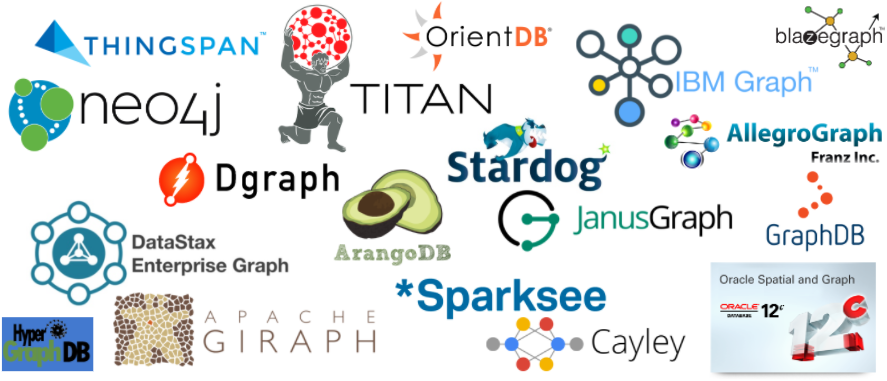
\includegraphics[scale=0.35]{immagini/graphdb.png}

	\caption{\textit{Alternative tecnologiche nel mercato \link{https://goo.gl/d3UUgT}}}
\end{figure}

\subsubsection{Sparksee(DEX)}
Sparksee\footnote{Sparksee: url= \link{http://www.sparsity-technologies.com/}} è un grafo nativo sviluppato in C++ da Spark Technologies a fine 2008 sotto nome DEX. Successivamente nel 2014 cambia nome in Sparksee.\\
È stato il primo \textit{database} a grafo disponibile per Android e iOS.\\
Supporta tecnologie di rilievo per l'azienda come Java, Maven e viene rilasciato per Linux, MacOs, Windows e per i principali sistemi operativi mobili.
La casa produttrice dichiara come caso d'uso possibile il rilevamento di frode bancarie.\\
Questa tecnologia viene rilasciata solamente in versione con licenza commerciale ed accademica con il limite ad un milione di nodi.

\subsubsection{Neo4j}
Neo4j\footnote{Neo4j: url= \link{https://neo4j.com/}} è la base di dati a \gls{grafo nativa} più diffusa al mondo, e, anche grazie a questo, ha una \textit{community} molto ampia. È un \textit{software} sviluppato in Java da Neo Technology nel 2007. È adottato da multinazionali come Microsoft, AirBnb, IBM, Ebay.\\
Neo4j ha un linguaggio di interrogazione proprietario, chiamato Chyper, molto espressivo e ottimizzato. Supporta le tecnologie di rilievo per l'azienda, compreso Spring Data\footnote{Spring data: url= \link{http://projects.spring.io/spring-data/}}. Neo4j viene rilasciato in versione \textit{community} gratuita con nessuna limitazione di ampiezza della base di dati senza la possibilità di eseguirlo in modo distribuito, al contrario di quella \textit{Enterprise} a pagamento.

\subsubsection{ArangoDB}
ArangoDB\footnote{ArangoDB: url= \link{https://www.arangodb.com/}} è un \textit{database} multi modello sviluppato in C++ nato nel 2011. È un \textit{database} principalmente documentale ma con collezioni che, raccogliendo la chiave di entrata e di uscita, simulano il funzionamento a grafo. Questo permette di organizzare i dati utilizzando il modello a grafo, documentale e chiave/valore.\\
Gli sviluppatori promettono la flessibilità data dalle base di dati multi modello e velocità paragonabile ai \textit{database} a grafo nativi.\\
ArangoDB ha un linguaggio di interrogazione proprietario simile ad \gls{SQL} e viene rilasciato in versione gratuita con limitazioni solo nell'ambito della sicurezza.
\subsubsection{AllegroGraph}
AllegroGraph\footnote{AllegroGraph: url= \link{https://franz.com/agraph/allegrograph/}} è un software per \textit{database} a grafo nativo sviluppato insieme agli \textit{standard} W3C\footnote{W3C: url= \link{https://www.w3.org/}} per il \textit{web} \gls{semantico}  nel 2004. Supporta tecnologie di interesse all'azienda ma non ha un linguaggio di interrogazione proprietario. Viene rilasciato solo con licenza commerciale a pagamento.
\subsubsection{OrientDB}
OrientDB\footnote{OrientDB: url= \link{http://orientdb.com/orientdb/}} è un \textit{software} per base di dati multi modello sviluppato in Java da uno sviluppatore italiano chiamato Luca Garulli\footnote{Luca Garulli: url= \link{https://www.linkedin.com/in/garulli}}. È un \textit{database} principalmente documentale ma, salvando attraverso tabelle gli indici fisici di inizio e fine dell'arco, riesce ad implementare anche il modello a grafo nativo. \\
Per scelta puramente commerciale hanno deciso di integrare un linguaggio di interrogazione molto simile a \gls{SQL}, limitando di molto l'espressività nelle ricerche nel modello a grafo. Viene rilasciato in versione sia a pagamento che \textit{community} con nessuna limitazione di rilievo.
\subsubsection{Titan}
Titan\footnote{Titan: url= \link{http://titan.thinkaurelius.com/}} è un software in grado di sfruttare \textit{storage backend} come Apache Cassandra\footnote{Apache Cassandra: url= \link{http://cassandra.apache.org/}} per l'immagazzinamento dei dati. È capace di astrarre i dati nello \textit{storage} ed organizzarli come se fossero a grafo, di conseguenza non utilizza una base di dati a \gls{grafo nativa}.
Questa possibilità di scelta dello \textit{storage backend} lo rende molto valido se l'azienda utilizzasse una tecnologia che lo supporta, questo porterebbe ad un costo di passaggio tecnologico più contenuto.\\
Titan non offre un linguaggio di interrogazione proprietario ma supporta pienamento Tinkerpop.  Viene rilasciato in licenza Apache 2\footnote{Apache 2: url= \link{https://www.apache.org/licenses/LICENSE-2.0}}.
\subsection{Scelta tecnologica}
\begin{figure}[h!]
	\centering
	
\includegraphics[scale=0.45]{immagini/neo4j.png}
	
\includegraphics[scale=0.3]{immagini/orientdb.png}
	\caption{\textit{Logo \href{https://neo4j.com/}{Neo4j} e \href{http://orientdb.com/orientdb/}{OrientDB}}}
\end{figure}
Dopo un colloquio dove ho mostrato al mio tutor i risultati dell'analisi, in comune accordo abbiamo scelto le due tecnologie più promettenti ed interessanti.\\
Abbiamo scelto \textbf{Neo4j} per il suo linguaggio di interrogazione molto espressivo e la sua diffusione a livello mondiale che porta ad una \textit{community} molto attiva.\\
Infine abbiamo scelto anche \textbf{OrientDB} essendo il \textit{database} multi modello più promettente sulla carta che organizza i dati come uno a grafo nativo.
\\
\\

\section{Sviluppo del prototipo}
\subsection{Analisi dei requisiti}
La prima attività svolta, dopo l'analisi delle tecnologie, è stata l'analisi dei requisiti. Questo perché l'organizzazione della base di dati deve essere strutturata in modo tale da semplificare le operazione che il prototipo andrà ad eseguire.\\
Ho tracciato tutti i requisiti utilizzando il seguente schema.\\
\begin{itemize}
	\item \textbf{Importanza:} può assumere questi valori:
  		\begin{itemize}
    		\item \textbf{1:} indica un requisito obbligatorio;
    		\item \textbf{2:} indica un requisito opzionale;
  		\end{itemize}
  	\item \textbf{Tipo:} può assumere questi valori:
  		\begin{itemize}
   		 	\item \textbf{F:} indica un requisito funzionale;
    		\item \textbf{Q:} indica un requisito di qualità;
    		\item \textbf{V:} indica un requisito di vincolo.
  		\end{itemize}
  	\item \textbf{Identificativo:} indica il codice identificativo del requisito, è un intero positivo crescente.
\end{itemize}
Ho definito tutti i requisiti tramite \textit{brainstorming} con il mio tutor aziendale e definiti nella seguente tabella.
\label{tab:rec}
\begin{table}[!ht]
\begin{tabularx}{\textwidth}{Xll}
\hline\hline
\textbf{Requisito} & \textbf{Identificativo} \\
\hline
Stesura documento con descrizione dettagliata dell'analisi svolta. & 1V1\\
\hline
Predisposizione di un ambiente di lavoro con il \textit{database} scelto utilizzando \textit{deploy} tramite container docker. & 1V2\\
\hline
Sviluppo prototipo & 1V3\\
\hline
Preparazione ed esecuzione di una presentazione. & 2V4\\
\hline
Estensione del \textit{dataset} considerato e aggiunta di maggiore complessità nelle relazioni valutate. & 2V5\\
\hline
Il prototipo deve permettere il calcolo della reputazione totale & 1F6\\
\hline
Il prototipo deve permettere il calcolo della reputazione relativa & 1F7\\
\hline
Il prototipo deve permettere l'aggiunta di una transazione & 1F8\\
\hline
Il prototipo deve permettere l'aggiunta di un \textit{AccountId} & 1F9\\
\hline
Il prototipo deve permettere l'aggiunta di un \textit{EntityId} & 1F10\\
\hline
Il prototipo deve permettere di associare un \textit{AccountId} ad un \textit{EntityId} & 1F11\\
\hline
Il prototipo deve permettere l'eliminazione di un \textit{AccountId} & 1F12\\
\hline
Il prototipo deve permettere l'eliminazione di un \textit{EntityId} & 1F13\\
\hline
La copertura dei test di unità deve essere maggiore o uguale al 85\% & 1Q14\\
\hline
Il prototipo deve permettere il calcolo dell'ammontare delle transazioni da una certa data in poi rispetto un \textit{AccountId} & 2F15\\
\hline
Il prototipo deve riuscire a calcolare la somma delle reputazioni totali di tutti gli \textit{AccountId} associati ad un \textit{EntityId} & 2F16\\
\hline
Il prototipo deve riuscire a calcolare la somma delle reputazioni relative di tutti gli \textit{AccountId} associati ad un \textit{EntityId} & 2F17\\
\hline
Soddisfacimento del 100\% dei requisiti obbligatori & 1F18\\
\hline
\end{tabularx}
\caption{Tabella tracciamento requisiti.}
\end{table}%
\\
Tutti i requisiti descritti sono stati poi approvati dal mio tutor aziendale.
\newpage
\subsection{Tecnologie utilizzate}
Tutte le tecnologie che ho utilizzato sono state accordate preventivamente con il tutor aziendale.
\subsubsection{IntellJ Idea Ultimate}
Ho utilizzato IntellJ Idea, con licenza accademica, come \gls{IDE} in primo luogo per la conoscenza maturata dai progetti passati eseguiti in ambito universitario. Inoltre integra il supporto a JUnit\footnote{JUnit: url= \link{http://junit.org/junit5/}} per facilitare i \textit{test}, a Maven per eseguire la \textit{Build} direttamente dall'\gls{IDE}, \textit{debugger} avanzato. In aggiunta offre anche molte funzionalità utili come la possibilità di eseguire \textit{\gls{refractoring}} con la certezza che il comportamento resti invariato.

\subsubsection{Java 8}
Ho utilizzato Java come linguaggio di programmazione perché, in primo luogo, era un vincolo dettato dal piano di lavoro descritto nella \hyperlink{sec:pianodl}{sezione 2.1.3}. Inoltre questo linguaggio ha una sintassi molto regolare e semplice. Infine essendo uno dei linguaggi più diffusi al mondo ha una vasta quantità di librerie supportate.
\subsubsection{Maven}
Maven\footnote{Maven: url= \link{https://maven.apache.org/}} è uno strumento per la gestione di progetti \textit{software} sviluppato da Apache Software Foundation\footnote{https://www.apache.org/}. Permette di dichiarare tutte le dipendenze e le varie versioni delle librerie in un unico file in formato XML\footnote{XML: url\link{https://it.wikipedia.org/wiki/XML}}, separando le \textit{directory} di progetto dalle librerie utilizzate. Maven scaricherà automaticamente le dipendenze e le nasconderà in cartelle separate dal progetto.\\
La \textit{build standard} automatica consiste in diversi passi ordinati e dipendenti l'uno dall'altro tra cui la compilazione, l'esecuzione dei \textit{test}, la verifica. Questo ciclo di \textit{build standard} sarà completato solamente se tutte la varie fasi non genereranno errori.
\begin{figure}[h!]
	\centering
	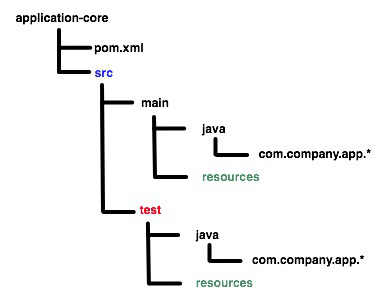
\includegraphics[scale=0.5]{immagini/maven.jpg}
	\caption{\textit{Struttura standard delle cartelle} \link{https://goo.gl/N94Uqs}}
\end{figure}
\subsubsection{Spring Boot}
\begin{figure}[h!]
	\centering
	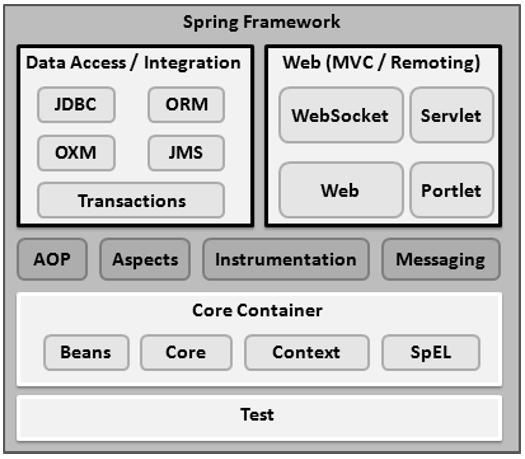
\includegraphics[scale=0.45]{immagini/spring.png}
	\caption{\textit{Architettura del \gls{framework} Spring} \link{https://goo.gl/2hvVYM}}
\end{figure}
Spring Boot\footnote{Spring Boot: url= \link{https://projects.spring.io/spring-boot/}} è un \gls{framework} per semplificare la creazione di progetti Java \textit{stand-alone}. Con questo \gls{framework} è possibile definire l'architettura interna di un progetto, ad esempio un \textit{web server}, con semplici annotazioni Java.\\
Per la creazione di un progetto Spring Boot basta recarsi in \link{https://start.spring.io/}, configurare il nome del progetto e scaricare il sorgente.\\
Spring è una valida alternativa a Enterprise JavaBeans\footnote{Enterprise JavaBeans: url= \link{https://it.wikipedia.org/wiki/Enterprise\textunderscore JavaBeans}}.

\subsubsection{Spring Data Neo4j}

Spring Data Neo4j\footnote{Spring Data Neo4j: url= \link{https://projects.spring.io/spring-data-neo4j/}} è una particolare implementazione di Spring Data\footnote{Spring Data: url= \link{http://projects.spring.io/spring-data/}}. Questa libreria permette di astrarre le operazioni che si eseguono nella base di dati Neo4j semplificando lo sviluppo.\\
Utilizzando questa libreria è possibile definire delle \textit{query} solo grazie alle segnatura dei metodi, questo permette sia velocizzare lo sviluppo sia l'attività di verifica visto che sarebbe inutile eseguirla in un metodo già verificato dalla casa produttrice. Infine permette di eseguire il \textit{map} degli oggetti Java nel \textit{database} semplicemente con delle annotazioni senza generazione di codice.
\begin{figure}[h!]
	\centering
	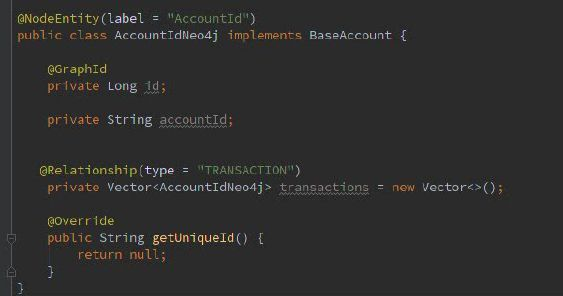
\includegraphics[scale=0.33]{immagini/sdata.jpg}
	\caption{\textit{Esempio di Nodo utilizzando Spring Data Neo4j}}
\end{figure}

\subsubsection{Tinkerpop}

Ho utilizzato Tinkerpop\footnote{Tinkerpop: url= \link{http://tinkerpop.apache.org/}} per interfacciarmi con OrientDB in modo semplice, diminuendo le operazioni eseguite esclusivamente tramite \textit{query}. Questa libreria ha il vantaggio di permettere un passaggio ad un'altra tecnologia che lo supporta senza modificare il codice. E stata sviluppata da Apache Software Foundation con lo scopo di uniformare il codice volto a interfacciarsi con la maggior parte dei \textit{database} nel mercato.
\begin{figure}[h!]
	\centering
	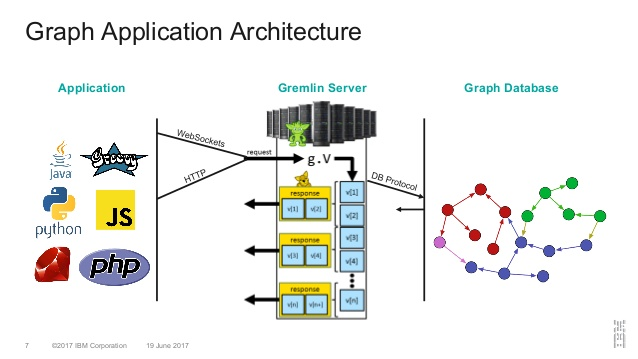
\includegraphics[scale=0.65]{immagini/tinkerpop.jpg}
	\caption{\textit{Architettura di un'applicazione che utilizza Tinkerpop} \link{https://goo.gl/YiXuLB}}
\end{figure}

\subsubsection{JUnit e Mockito}
JUnit\footnote{JUnit: url= \link{http://junit.org/junit5/}} è un \gls{framework} che permette e semplifica la creazione di test in Java. Invece Mockito\footnote{Mockito: url= \link{http://site.mockito.org/}} permette di sovrascrivere il comportamento di un particolare metodo impostandogli i valori di entrata e di uscita. Questo è utile quando si sviluppano i \textit{test} di unità e si utilizzano delle particolari classi non sviluppate o semplicemente non coperte da \textit{test}.
\newpage
\begin{figure}[h!]
	\centering
	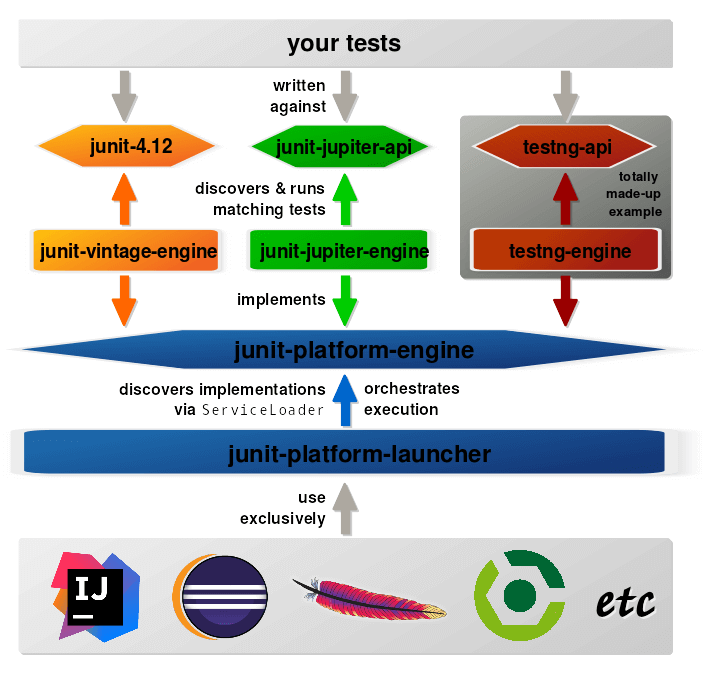
\includegraphics[scale=0.27]{immagini/junit.png}
	
	\caption{\textit{Architettura di JUnit \link{https://goo.gl/6Xgy5U}}}
\end{figure}




\subsection{Base di dati}
In base al problema descritto nella \hyperref[sec:prob]{sezione 2.1.1}, dinamiche di Smash\textregistered\ ed i requisiti descritti nella \hyperref[tab:rec]{tabella 3.1} ho organizzato i dati, per tutti e due i \textit{database}, nel seguente modo:
\begin{itemize}
\item{\textbf{Nodi:}}
\begin{itemize}
\item{\textbf{EntityId:}} è il nodo che rappresenta un utente di una banca, esso può sia svolgere transazioni verso un \textit{AccountId} che avere relazioni di appartenenza verso uno, o più, \textit{AccountId}.
\item{\textbf{AccountId:}} è il nodo che rappresenta una coordinata bancaria ad esempio un iban, esso può avere transazioni verso altri \textit{AccountId} ed avere massimo una relazione di appartenenza da un \textit{EntityId} a questo nodo.
\end{itemize}
\item{\textbf{Archi:}}
\begin{itemize}
\item{\textbf{TRANSACTION:}} è l'arco che rappresenta una transazione, questo può provenire da un \textit{AccountId} o \textit{EntityId} verso un \textit{AccountId}. Questo ha diverse proprietà tra cui di obbligatorie la data di avvenuta transazione, l'importo e la valuta, e di non obbligatorie come la città e il paese dove è stata eseguita la transazione.
\item{\textbf{OWN:}} è l'arco che descrive la relazione di appartenenza da un \textit{EntityId} ad un \textit{AccountId}. Un \textit{EntityId} può avere un numero a piacere di relazioni di appartenenza, al contrario un \textit{AccountId} può avere al massimo un arco entrante di tipo \textit{OWN}.
\end{itemize}
\end{itemize}
\newpage
\begin{figure}[!ht]
	\centering
	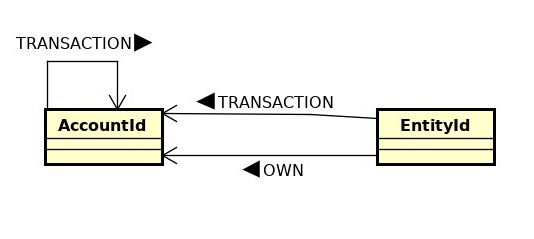
\includegraphics[scale=0.4]{immagini/graph.jpg}
	\caption{\textit{Schema della base di dati}}
\end{figure}
A causa dei problemi legati alle politiche della protezione dei dati sensibili, non ho potuto utilizzare dati reali per il popolamento dei \textit{database} ma ho dovuto creare un progetto per la generarmeli in modo casuale.
\subsection{Prototipo}
\begin{figure}[h!]
	\centering
	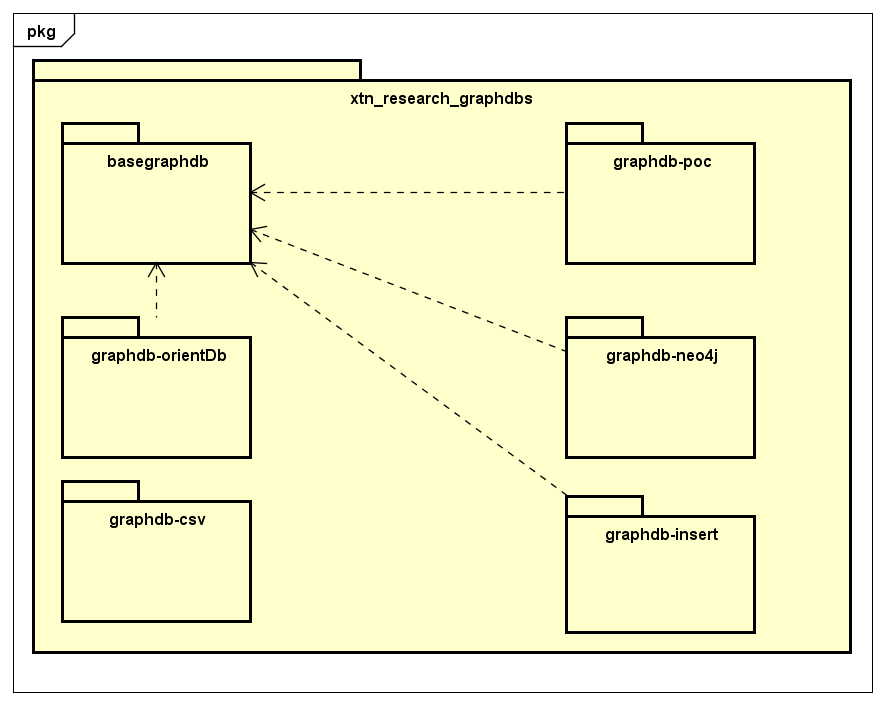
\includegraphics[scale=0.4]{immagini/packages.png}
	\caption{\textit{Diagramma dei package del prototipo}}
\end{figure}
Ho deciso di dividere il prototipo in più progetti sotto l'unico \gls{aggregato Maven} chiamato \textit{xtn\textunderscore research\textunderscore graphdbs}. Questa tecnica l'ho utilizzata per gestire tutte le versioni delle dipendenze in un unico file di configurazione, e, sopratutto, per avere la comodità di eseguire la \textit{build} di tutti i progetti in un unico comando, lasciando a Maven l'onere di risolvere tutte le dipendenze.\\


\subsubsection{basegraphdb}
\textit{Basegraphdb} é il progetto che contiene le varie interfacce comuni tra cui \textit{ReputationController}. Questa é l'interfaccia comune per gestire la reputazione delle varie entitá presenti nei vari \textit{database}. Ogni implementazione, quindi sia \textit{graphdb-neo4j} che \textit{graphdb-orientDb}, conterrà una classe che la implementerà.
\subsubsection{graphdb-orientdb}
\textit{Graphdb-orientDb} é il progetto per la gestione della reputazione tramite OrientDB, esso ha all'interno una classe chiamata \textit{ReputationControllerOrientDb} che implementa \textit{ReputationController}. Questa implementazione usa Tinkerpop\footnote{Tinkerpop: url=\link{http://tinkerpop.apache.org/}} per interfacciarsi con il \textit{database}.
\subsubsection{graphdb-neo4j}
\textit{Graphdb-neo4j} è il progetto per la gestione della reputazione tramite Neo4j, esso ha all'interno una classe chiamata \textit{ReputationControllerNeo4j} che implementa \textit{ReputationController}. Questa implementazione utilizza \textit{Spring Data Neo4j} per interfacciarsi ed eseguire il \textit{map} degli oggetti Java nel \textit{database}.


\subsubsection{graphdb-csv}
\textit{Graphdb-csv} è il progetto per creare tutti i documenti in formato CSV contenenti le entità per popolare i diversi tipi di \textit{database}. Questo crea dati in modo casuale nei migliori dei casi, cioè ogni \textit{AccountId} ha il proprio \textit{EntityId}.\\

\subsubsection{graphdb-insert}
\textit{Graphdb-insert} inserisce in modo del tutto causale un certo numero, definito dall'utente, di \textit{EntityId, AccountId, Transaction} utilizzando l'interfaccia comune \textit{ReputationController}.\\
\textbf{Questo progetto deve essere usato solo per inserire un modesto numero di nodi ed archi} visto che l'aggiunta di ogni \textit{record} ci impiega 500 millisecondi. In caso contrario è consigliato generarsi i CSV delle entità utilizzando il progetto \textit{graphdb-csv} e successivamente importarli nel \textit{database} scelto.
\subsubsection{graphdb-poc}
\textit{Graphdb-poc} è il progetto che si occupa solamente di instanziare le varie implementazioni di \textit{ReputationController} ed eseguire i vari metodi d'interfaccia tracciando, e stampando a video, il nome del metodo, il risultato ottenuto ed il tempo impiegato.\\
Questo progetto non ha dipendenze verso le varie implementazioni ma solamente verso l'interfaccia. Questo è possibile delegando a Spring l'onere di iniettare tutte le classi che implementano l'interfaccia comune. In questo modo si ha un disaccoppiamento tra questo progetto e le varie implementazioni e, sopratutto, se in futuro ci fosse il bisogno di aggiungerne un altra non sarebbe necessario modificare il codice di questo progetto.
\begin{figure}[!ht]
	\centering
	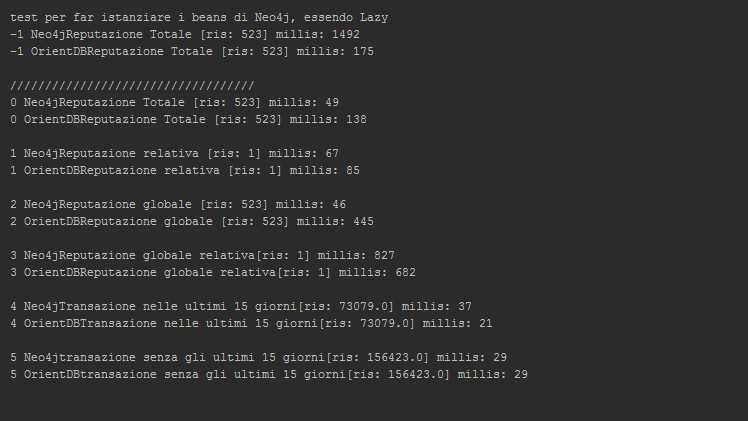
\includegraphics[scale=0.75]{immagini/poc.png}
	\caption{\textit{Risultati stampati da graphdb-poc}}
\end{figure}
\newpage
\section{Utilizzo della libreria}
\subsection{Calcolo della reputazione}
Sfruttando la \textit{dependency injection} \footnote{dependency injection: url= \link{https://en.wikipedia.org/wiki/Dependency\textunderscore injection}} di Spring, per utilizzare la libreria del calcolo della reputazione è sufficiente creare una classe simile alla seguente.
\begin{lstlisting}
package it.ldario;

import it.ldario.graphdbneo4j.ReputationControllerNeo4j;
//import it.ldario.graphdborientDb.ReputationControllerOrientDb;
import org.springframework.beans.factory.annotation.Autowired;
import org.springframework.boot.CommandLineRunner;
import org.springframework.boot.SpringApplication;
import org.springframework.boot.autoconfigure.SpringBootApplication;

@SpringBootApplication
public class MiaClasse implements CommandLineRunner {

    public static void main(String[] args) {
        SpringApplication.run(MiaClasse.class, args);
    }
    
    
	
	//utilizzando, come tipo statico, ReputationControllerNeo4j oppure //ReputationControllerOrientDb verra' usato, rispettivamente //l'implementazione di Neo4j o OrientDB
    private ReputationControllerNeo4j reputationController;
    //private ReputationControllerOrientDb reputationController;



    @Autowired
    public MiaClasse(ReputationControllerNeo4j reputationController) {
        this.reputationController = reputationController;
    }
    

    @Override
    public void run(String... strings) throws Exception {
        //aggiunge al database scelto(orientDB oppure Neo4j), dipende dal tipo //che viene dichiarato, un entity con id="Luca"
        reputationController.addAccountId("Luca");

        //stampa la reputazione totale dell'entity "Luca"
        System.out.println(reputationController.getTotalReputation("Luca"));
        
        

        //stampa il totale delle transazioni effettuate da Luca negli ultimi //15 giorni
		System.out.println(reputationController
        						.getAmountAccountIdInATimeRange("Luca", 15));
        						
        						
        						
        //aggiunge al database scelto(orientDB oppure Neo4j), dipende dal tipo //che viene dichiarato, un account con id "IT123"
        
         TransactionBuilder transactionBuilder = new TransactionBuilder(); 
        transactionBuilder.setCountry("Italy").setCity("San Michele delle Badesse").setAmount(100).setCurrency("Euro");
        reputationController.addTransaction("Luca","IT123",transactionBuilder
        																.build());
        

    }
}
\end{lstlisting}
\subsection{Estensione della libreria con un altro tipo di database}
Per aggiungere un altro tipo di database è necessario solamente creare una classe simile alla seguente, senza modificare il codice del prototipo.
\begin{lstlisting}
package it.ldario.newdatabase;

import it.ldario.basegraphdb.ReputationController;


public class ReputationControllerNewDatabase implements ReputationController {
    //implementazione di tutti i metodi di interfaccia
}
\end{lstlisting}

\subsection{Popolamento della base di dati}
Per aggiungere un numero modesto di dati generati casualmente, in qualunque tecnologia che implementa \textit{ReputationController}, è necessario solamente creare una classe simile alla seguente.
\begin{lstlisting}
package it.ldario;


import it.ldario.graphdbinsert.GraphDbInsertImpl;
import it.ldario.graphdbneo4j.ReputationControllerNeo4j;
//import it.ldario.graphdborientDb.ReputationControllerOrientDb;
import org.springframework.beans.factory.annotation.Autowired;
import org.springframework.boot.CommandLineRunner;
import org.springframework.boot.SpringApplication;


public class MiaClasse implements CommandLineRunner {

    //esplicitando il tipo verra' scelto, rispettivamente, il reputation //controller di Neo4j o OrientDB
    private ReputationControllerNeo4j reputationController;
    //private ReputationControllerOrientDb reputationController;

    public static void main(String[] args) {
        SpringApplication.run(GraphdbPocApplication.class, args);
    }

    @Autowired
    public MiaClasse(ReputationControllerNeo4j reputationController) {
        this.reputationController = reputationController;
    }

    @Override
    public void run(String... strings) throws Exception {
        GraphDbInsertImpl graphDbInsert = new GraphDbInsertImpl(10,20,50,reputationController);

    }
}
\end{lstlisting}
Eseguendo il \textit{Main} si andranno ad aggiungere nel \textit{database} scelto 10 \textit{EntityId}, 20 \textit{AccountId} e 50 Transazioni. Per scegliere la base di dati su cui agire è necessario modificare, con il tipo desiderato, la variabile \textit{reputationController}.




\section{Verifica e validazione}
\subsection{Verifica}
Nell'attività di verifica ho utilizzato JUnit\footnote{JUnit: url= \link{http://junit.org/junit5/}} e Mockito\footnote{Mockito: url= \link{http://site.mockito.org/}} per facilitare la creazione dei \textit{test}.

\begin{figure}[!ht]
	\centering
	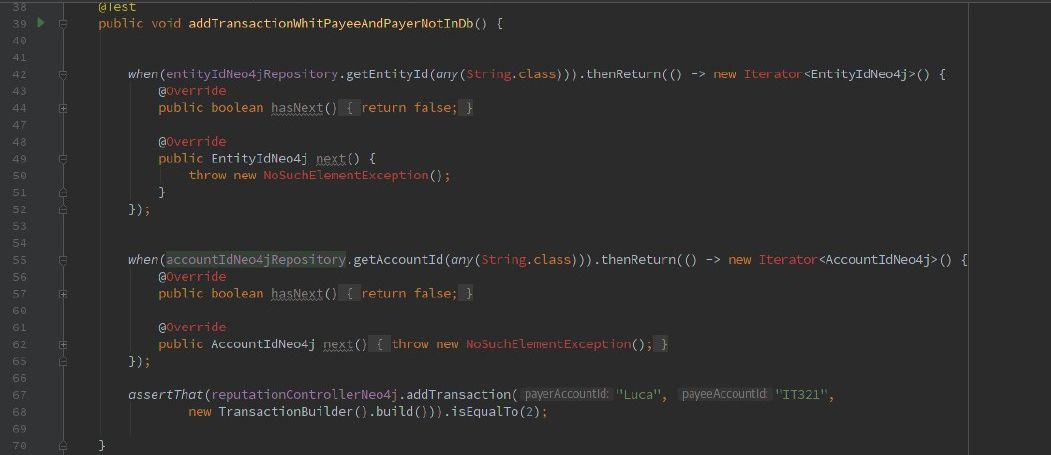
\includegraphics[scale=0.4]{immagini/test.jpg}
	\caption{\textit{Esempio di test utilizzando Mockito e JUnit}}
\end{figure}
Sono state testate tutte le \textit{query} utilizzando un immagine docker\footnote{Docker: url= \link{https://www.docker.com/}} di \textit{test}, escluse quelle banali auto generate da Spring.
Invece per testare le varie unità mi sono aiutato istanziando ed istruendo facilmente dei \textit{mock} utilizzando Mockito.
In accordo con il mio tutor aziendale è stata decisa la soglia minima di copertura dei test del 85\%.\\
La copertura finale dei test si è attestata sul 88\% tra il codice consegnato in azienda.
Ogni test ha uno ed uno solo confronto al suo interno ed ha un nome che indica con precisione che operazioni andrà ad eseguire. Questo ha il vantaggio di sapere esattamente con che condizioni il \textit{test} fallisce solamente leggendo il nome. Inoltre ogni requisito è stato coperto da \textit{test}, questo per verificare l'avvenuto soddisfacimento di esso.\\
Tutti i \textit{test} verificano la logica interna dell'unità e percorrono la quasi totalità dei cammini possibili, questo per far emergere tutti i possibili errori nel codice.
\newpage
\begin{figure}[!ht]
	\centering
	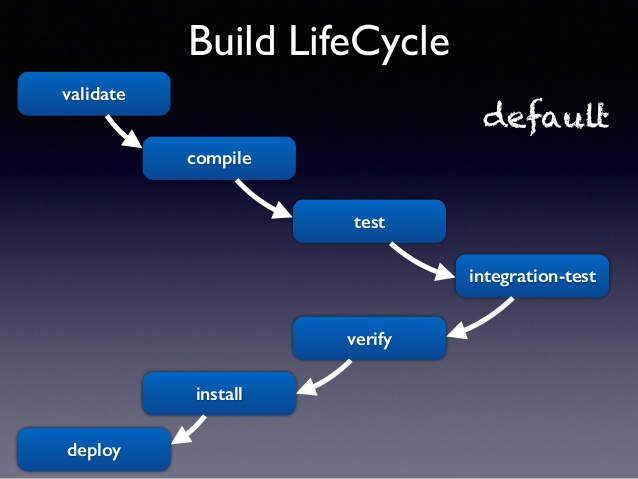
\includegraphics[scale=0.4]{immagini/build.jpg}
	\caption{\textit{Ciclo di vita della build standard di Maven \link{https://goo.gl/gvgZBN}}}
\end{figure}

La \textit{build} non andrà a buon fine se tutti i \textit{test} non avranno esito positivo, questo è gestito completamente e garantito dal processo di \textit{build standard} di Maven.
\subsection{Validazione}
\label{sec:valid}
Per quanto riguarda la validazione ho consegnato un documento, in azienda, contenente una tabella con il codice del requisito descritto nella \hyperlink{tab:rec}{tabella 3.1} e se è stato soddisfatto.\\
La tabella dei riquisiti obbligatori è la seguente:

\label{tab:pian}
\begin{table}[!ht]
\begin{tabularx}{.35\textwidth}{XX}
\hline\hline
\textbf{Requisito} & \textbf{S\footnote{S: Soddisfatto}/NS\footnote{NS: Non soddisfatto}} \\
\hline
1V1 & S\\
\hline
1V2 & S\\
\hline
1V3 & S\\
\hline
1F6 & S\\
\hline
1F7 & S\\
\hline
1F8 & S\\
\hline
1F9 & S\\
\hline
1F10 & S\\
\hline
1F11 & S\\
\hline
1F12 & S\\
\hline
1F13 & S\\
\hline
1Q14 & S\\
\hline
1F18 & S\\
\hline
\end{tabularx}
 \captionsetup{singlelinecheck = false, format= hang, justification=raggedright}
\caption{Tabella soddisfacimento requisiti obbligatori}
\end{table}%
\newpage
Invece la tabella dei requisiti opzionali è la seguente:


\label{tab:pian1}
\begin{table}[!ht]
\begin{tabularx}{.35\textwidth}{XX}
\hline\hline
\textbf{Requisito} & \textbf{S\footnote{S: Soddisfatto}/NS\footnote{NS: Non soddisfatto}} \\
\hline
2V4 & S\\
\hline
2V5 & NS\\
\hline
2F15 & S\\
\hline
2F16 & S\\
\hline
2F17 & S\\
\hline
\end{tabularx}
 \captionsetup{singlelinecheck = false, format= hang, justification=raggedright}
\caption{Tabella soddisfacimento requisiti opzionali}
\end{table}%
Il requisito segnato con l'identificativo 2V5, cioè l'estensione del \textit{dataset}, non è stato soddisfatto per mancanza di tempo. Ho preferito consumare il tempo rimanente per eseguire una buona presentazione interna all'azienda. Ho soddisfatto il 100\% dei requisiti obbligatori e l'80\% di quelli opzionali.
\section{Conclusioni}
\subsection{Casi d'uso di una base di dati a grafo}
Durante la mia analisi mi sono reso conto di come una base di dati a grafo non possa essere utilizzata per immagazzinare qualunque tipo di dato, anzi gli usi sono molto ristretti. Un \textit{database} di questa tipologia è rivolto a chi deve salvare un altissimo numero di dati legato ad una cerchia di entità, di numero minore rispetto a questi. Solitamente questo altissimo numero di dati rappresentano gli archi e le entità rappresentano i nodi.\\
Questo succede perché le potenzialità delle basi di dati di questo tipo emergono quando si ha un alto numero di archi collegati ad un modesto numero di nodi. Se avesse l'esatto opposto, quindi molti vertici e pochi archi, le operazioni disponibili sull'attraversamento tra i nodi si ridurrebbero di molto.
Inoltre una base di dati di questo tipo non è adatta per operazioni che coinvolgono tutto il \textit{database}.\footnote{\textit{The good and the bad about graph databases} : url= \link{https://goo.gl/bRMwnv}}
\label{fig:social}
\begin{figure}[!ht]
	\centering
	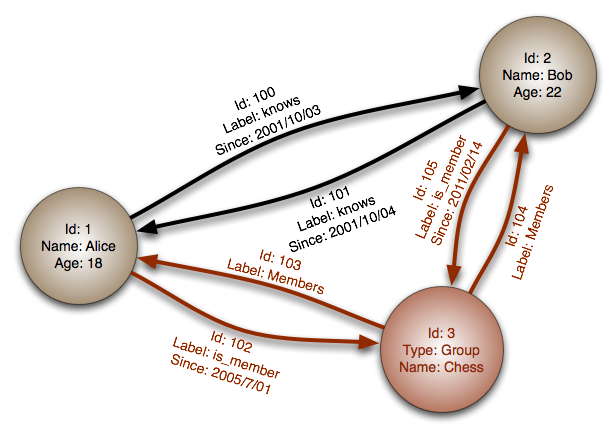
\includegraphics[scale=0.43]{immagini/social.png}
	\caption{\textit{Base di dati per un social network \link{https://goo.gl/Fik4Xp}}}
\end{figure}
\newpage
Un esempio classico di ottimo caso d'uso è quello descritto dalla \hyperlink{fig:social}{figura 3.8}, ossia la modellazione della base di dati di un social network. In questo caso il numero dei nodi, cioè le persone fisiche, sono in numero nettamente minore rispetto alla somma di tutti gli archi, cioè le conoscenze. Inoltre le operazioni che si eseguono coinvolgono sempre una base di dati circoscritta.\\

\subsection{Vantaggi e svantaggi di una base di dati a grafo}
Durante la mia analisi ho riscontrato i seguenti vantaggi e svantaggi nell'utilizzare una base di dati a grafo.
\subsubsection{Vantaggi}
\begin{itemize}
\item{\textbf{Velocità:}} se il caso d'uso è adatto e si organizzano i dati in modo intelligente si riesce a ridurre la maggior parte delle \textit{query} ad operazioni banali, sfruttando la natura dei grafi. Nell'ambito anti frode molte operazioni si riducono al "\textit{conta quante volte la persona \textbf{A} ha fatto una determinata cosa, chiamata \textbf{Z}, verso un entità \textbf{B}}" dove A e B sono nodi e Z è l'arco che li collega.
\item{\textbf{Espressività della ricerca:}} se il caso d'uso che si va a modellare è adatto alla natura dei grafi, l'espressività della ricerca è tale che le \textit{query} risultano, molte volte, banali anche dal punto di vista della scrittura.
\item{\textbf{Tutto è collegato:}} data dalla natura dei grafi, si ha un enorme possibilità di creare ricerche che esplorano in profondità il grafo date determinate condizioni, ad esempio la possibilità di attraversare e memorizzare solo i nodi che sono collegati da una determinata entità solamente tramite relazioni di appartenenza. Nell'ambito anti frode succede molto spesso di eseguire delle ricerche che sfruttano questa caratteristica.
\end{itemize}
\subsubsection{Svantaggi}
\begin{itemize}
\item{\textbf{Casi d'uso limitati:}} solo pochi \textit{use case} sono adatti ad essere modellati come un grafo, quindi è molto rischioso modellare totalmente la propria base di dati utilizzando questa tecnologia. Questo perché in futuro potrebbe esserci la necessità di aggiungere dati al modello non adatti a questo tipo di \textit{database}. Questo limita il normale ciclo di vita di un \textit{software}.
\item{\textbf{Tecnologia di nicchia:}} essendo una tecnologia di nicchia la possibilità di informarsi, tramite community, è ridotta rispetto ad altre tecnologie più diffuse, come possono essere i \textit{database} relazionali.
\end{itemize}
\newpage
\begin{figure}[!ht]
	\centering
	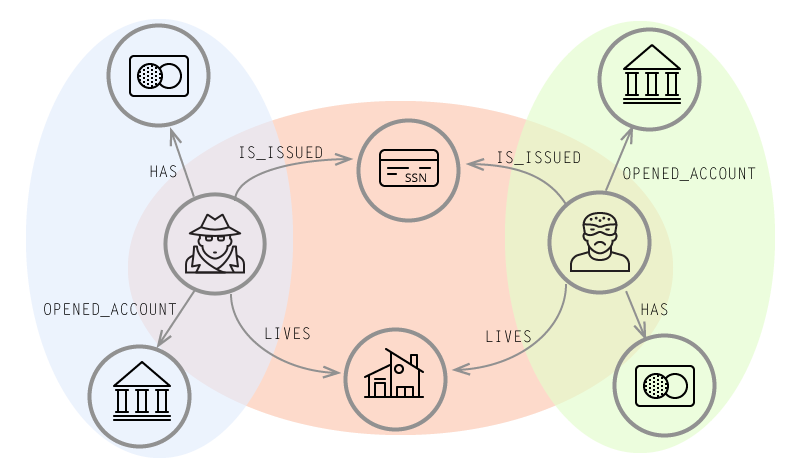
\includegraphics[scale=0.33]{immagini/fraud.png}
	\caption{\textit{Esempio di un caso d'uso orientato all'anti frode \link{http://archive.is/LpXtZ}}}
\end{figure}


\subsection{PRO e CONTRO Neo4j rispetto OrientDB}
\subsubsection{PRO}
\begin{itemize}
\item{\textbf{Espressività:}} chyper, il linguaggio di interrogazione di Neo4j, inizialmente può spaventare, essendo diverso da quelli che siamo abituati a vedere. Dopo un breve periodo di apprendimento risulta, però, facile da utilizzare e molto potente nelle ricerche. Questo è dato dalla sintassi molto regolare ed espressiva con pochissime nozioni.
\item{\textbf{Spring Data Neo4j:}} libreria ben fatta e documentata per astrarre l'interazione con la base di dati, al contrario di OrientDB.
\item{\textbf{Importatore da CSV:}} popolamento della base di dati tramite documento CSV nettamente più veloce rispetto ad OrientDB.
\end{itemize}
\subsubsection{CONTRO}
\begin{itemize}
\item{\textbf{Input/Output lento:}} le librerie di Neo4j, quali Spring Data ed in generale i \textit{driver} java, risultano più lenti rispetto ad quelli di OrientDB. Questo l'ho notato calcolando la differenza tra la velocità netta delle \textit{query}, eseguendola nella \textit{dashboard}, e quella tramite i \textit{driver}, successivamente confrontandola con OrientDB.
\end{itemize}
\subsection{PRO e CONTRO OrientDB rispetto Neo4j}
\subsubsection{PRO}
\begin{itemize}
\item{\textbf{Velocità:}} pur essendo un \textit{database} multi modello la velocità nelle ricerche è comparabile ad una base di dati a grafo.
\end{itemize}
\subsubsection{CONTRO}
\begin{itemize}
\item{\textbf{Spring Data OrientDB:}} non documentato ed acerbo. Questo mi ha portato ad usare Tinkerpop\footnote{Tinkerpop: url= \link{http://tinkerpop.apache.org/}} portando allo sviluppo di un software meno organizzato rispetto a quello di Neo4j.
\item{\textbf{Espressività:}} l'azienda produttrice di OrientDB ha fatto la scelta, per me puramente commerciale, di utilizzare un linguaggio simile ad \gls{SQL} per l'interrogazione della base di dati. Questo diminuisce sostanzialmente l'espressività delle \textit{query}, rendendo complicato lo sviluppo di operazioni con svariate transazioni su archi.
\item{\textbf{Spazio su disco:}} per rendere un database multi modello nativo gli sviluppatori di OrientDB hanno dovuto replicare molti dati, aumentando di circa 0.4 volte lo spazio necessario per immagazzinare i dati (prova eseguita con 30 milioni di record tra nodi ed archi).
\end{itemize}

\subsection{Conclusioni}
Nella parte finale del progetto di stage mi sono posto le seguenti domande per cercare di effettuare una presentazione esaustiva, in azienda, dell'analisi effettuata.\\
\\
\textbf{Vale la pena adottare la base di dati a grafo in azienda?}\\
\textit{Secondo la mia analisi si, però solamente per alcuni casi d'uso.}\\
Adottare un \textit{database} a grafo, e modellare i dati di conseguenza, per determinati casi d'uso renderebbero possibili determinate ricerche che prima potevano risultare troppo onerose o, addirittura, impossibili.\\
Il tratto caratteristico dei \textit{database} a grafo è la possibilità di attraversare, a costo costante, le varie entità ricostruendo le azioni compiute da una particolare entità indipendentemente dalla grandezza della base di dati. Questo aprirebbe, per l'azienda, nuove possibili ricerche come la costruzione dell'albero delle transazioni, dato un utente, per estrapolare determinate informazioni.\\
\\
\textbf{Risolve il problema iniziale del calcolo della reputazione descritto nella \hyperlink{sec:prob}{sezione 2.1.1}?}\\
\textit{Si, almeno utilizzando la base di dati generata casualmente.}\\
Ho eseguito le operazioni in basi di dati con varie unità di grandezza, fino ad arrivare a 30 milioni di transazioni, e il tempo necessario per calcolare la reputazione si aggirava tra i 2 millisecondi per quella totale e i 15 millisecondi per quella relativa. Questo grazie alla possibilità di eseguire queste determinate operazioni senza caricare tutto il \textit{database} in memoria.\\
\\
\\
\textbf{Quale tecnologia utilizzare tra Neo4j e OrientDB?}\\
\textit{Secondo la mia analisi Neo4j.}\\
Ho preso questa decisione analizzandoli nei seguenti 3 ambiti, in ordine di importanza:
\begin{itemize}
\item{\textbf{Espressività:}} il linguaggio di interrogazione di Neo4j è nettamente migliore in termini di espressività. SQL è chiaramente un linguaggio non adatto per le ricerche nei grafi. Al contrario, quello di Neo4j, è sempre espressivo sia in termini di lettura di una \textit{query} sia nel crearla. Questo rende meno costoso, in termini di studio, il cambio tecnologico in azienda. 
\item{\textbf{Supporto alle tecnologie usate in azienda:}} il passaggio a Neo4j risulterebbe meno costoso, in termini di studio individuale, grazie al supporto nativo verso Spring Data. Il supporto di OrientDB verso questa tecnologia risulta ancora acerbo.

\item{\textbf{Velocità:}} in termini di velocità di esecuzione di una \textit{query} Neo4j risulta migliore, sopratutto all'aumentare delle transazioni sui nodi.
\end{itemize}















